\subsection{Checking with MLP method}
\label{MLP_check}

Here we replace BDTG method with MLP method to replay the result in Figure \ref{fig:result_B_E}. The configuration of the MLP method is \texttt{factory->BookMethod( MVA::Types::kMLP, "MLP", "!H:!V:VarTransform=Norm:NeuronType=tanh:NCycles=500:HiddenLayers=N+20:\\TestRate=6:TrainingMethod=BFGS:Sampling=0.3:SamplingEpoch=0.8:\\ConvergenceImprove=1e-6:ConvergenceTests=15:!UseRegulator" )}.
From the result in Figure \ref{fig:MLP_B_E} one can see the MLP method also works but comparing with BDTG method its resolution is worse than BDTG method.
\begin{figure}[bh]
  \begin{center}
    \begin{tabular}{cc}
      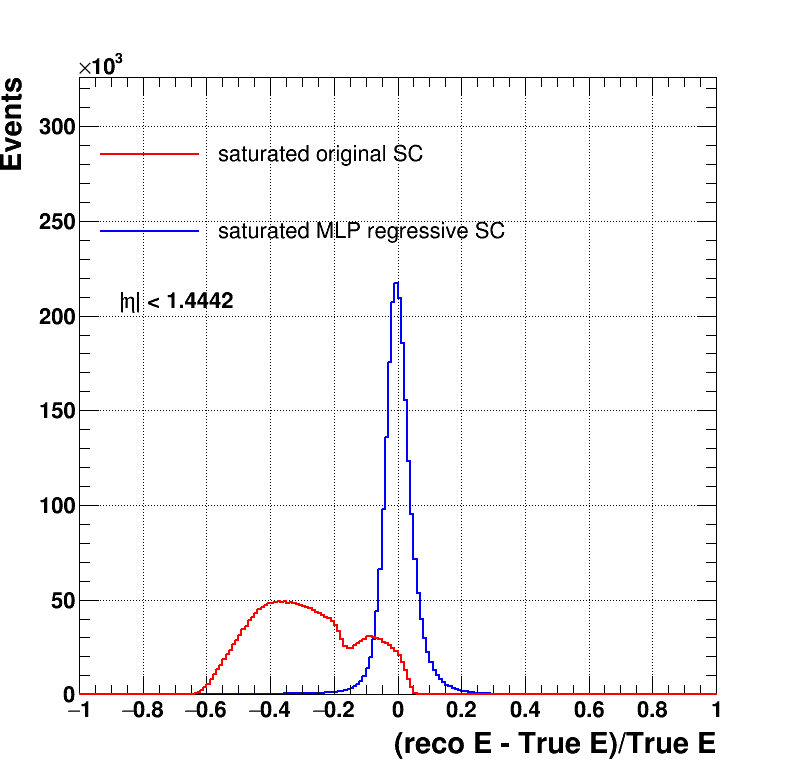
\includegraphics[width=0.45\textwidth]{chapters/Zprime/Saturation/images/FlatPt/check_MLP/compare_MLP_Barrel_Endcap_enSC_B_s.png} &
      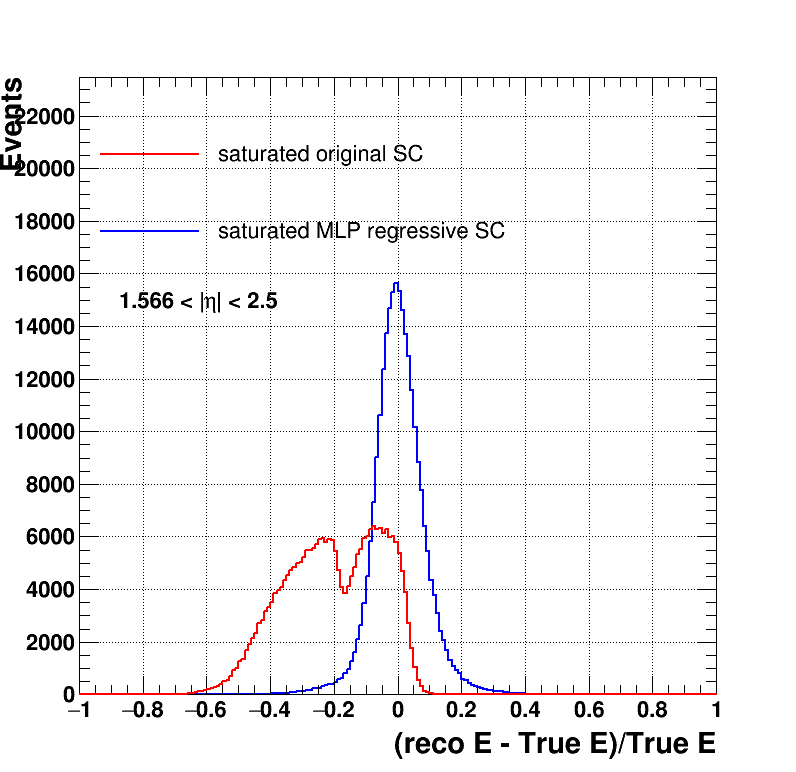
\includegraphics[width=0.45\textwidth]{chapters/Zprime/Saturation/images/FlatPt/check_MLP/compare_MLP_Barrel_Endcap_enSC_E_s.png} \\
      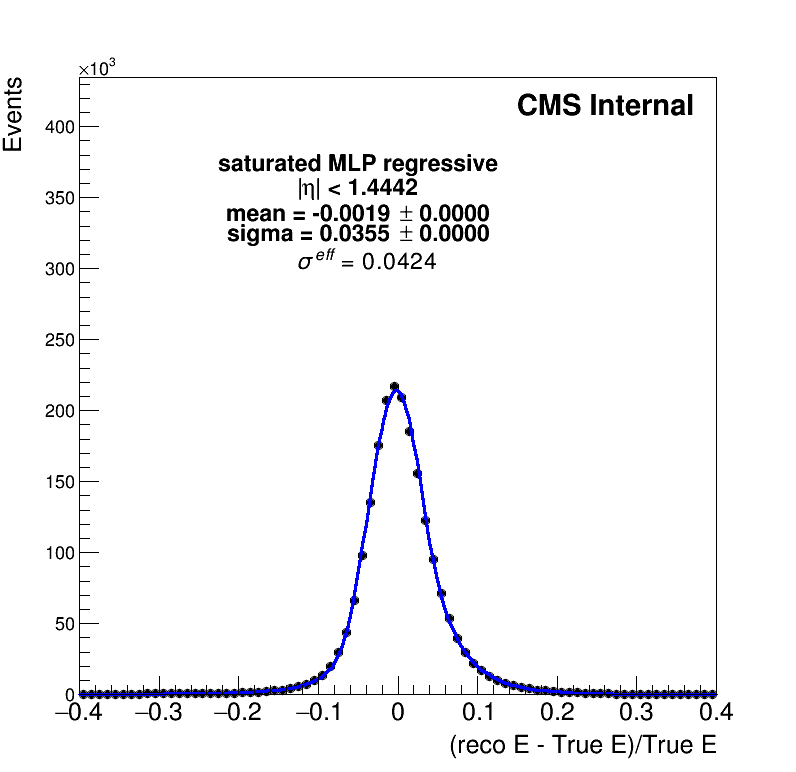
\includegraphics[width=0.45\textwidth]{chapters/Zprime/Saturation/images/FlatPt/check_MLP/fit_MLP_Barrel_Endcap_B_reg_s.png} &
      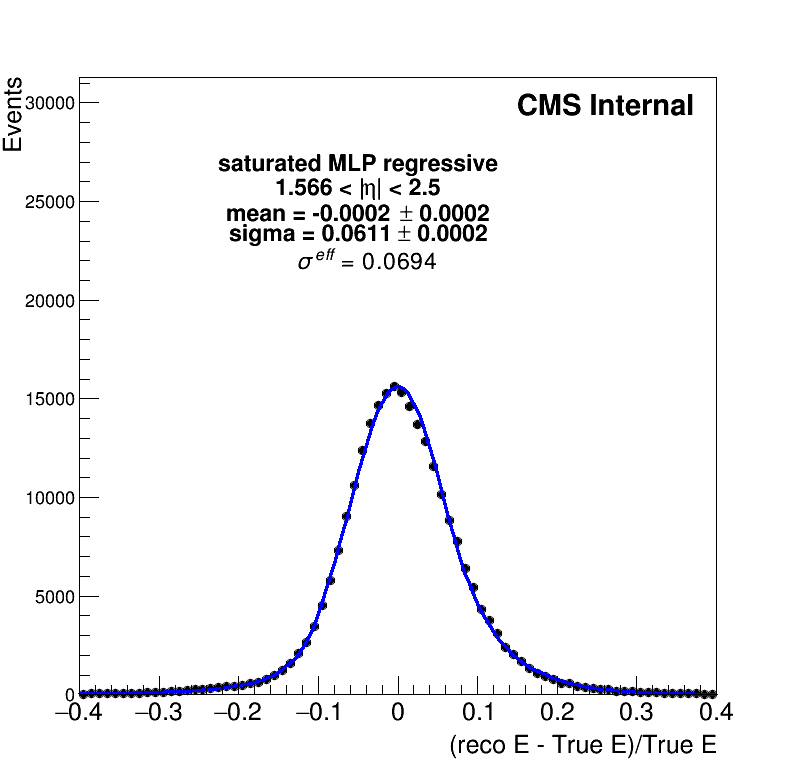
\includegraphics[width=0.45\textwidth]{chapters/Zprime/Saturation/images/FlatPt/check_MLP/fit_MLP_Barrel_Endcap_E_reg_s.png}
    \end{tabular}
    \caption{ The top plots are the distribution of supercluster energy minus ture energy divided by true energy for saturated electron for barrel (left) and endcap (right), the red histogram is for reconstructed supercluster enery, the blue histogram is for MVA regressive energy. The bottom plots are the fit of the blue histogram for barrel (left) and endcap (right).}
    \label{fig:MLP_B_E}
  \end{center}
\end{figure}
